\appendix
\section{Artifacts from Participatory Design\label{apdx:pdartifact}}
\begin{figure}[h!]
	\centering
	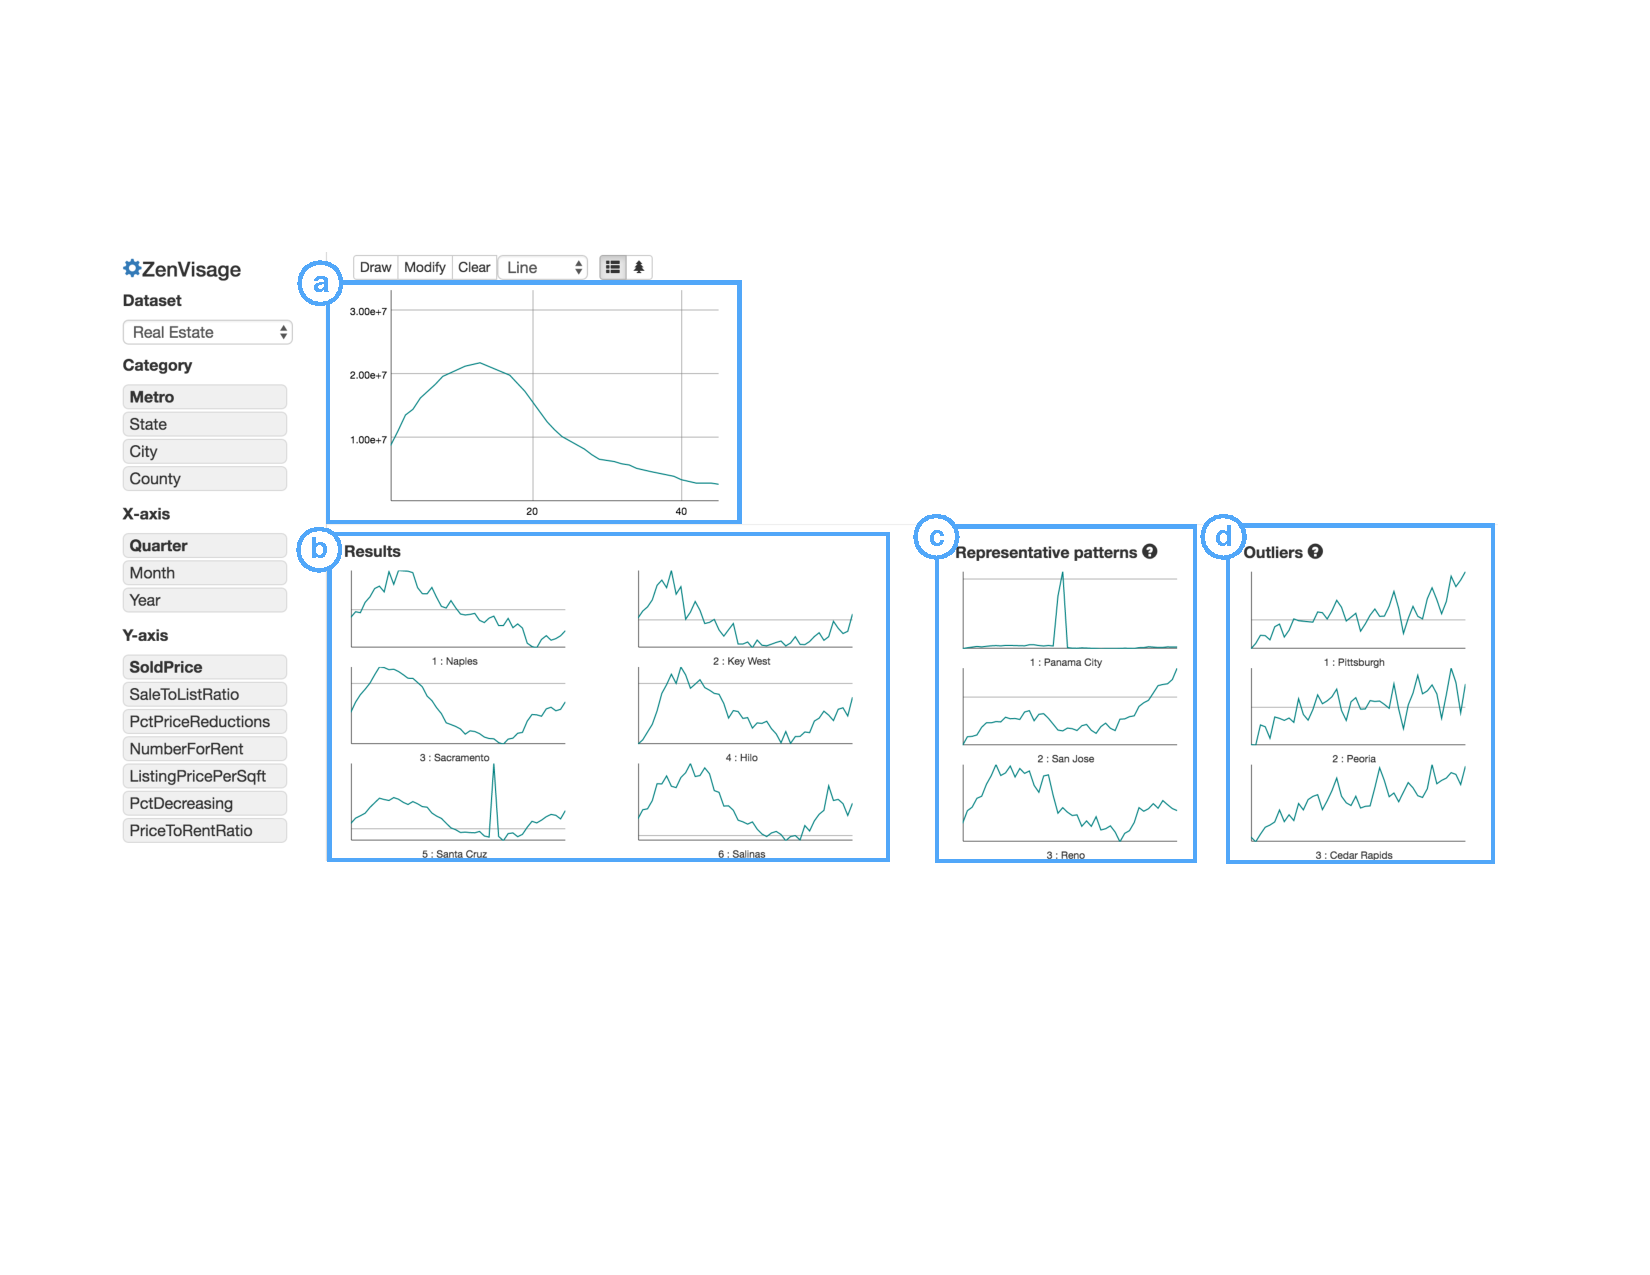
\includegraphics[width=\linewidth]{figures/oldZV_nozql.pdf}
	\caption{The existing \zv prototype allowed users to sketch a pattern in (a), which would then return (b) results that had the closest Euclidean distance from the sketched pattern. The system also displays (c) representative patterns obtained through K-Means clustering and (d) outlier patterns to help the users gain an overview of the dataset.}
	\label{oldZV}
\end{figure}

\begin{figure*}[ht!]
	\centering
	\captionsetup{justification=centering,margin=2cm}
	\vspace{-10pt}
	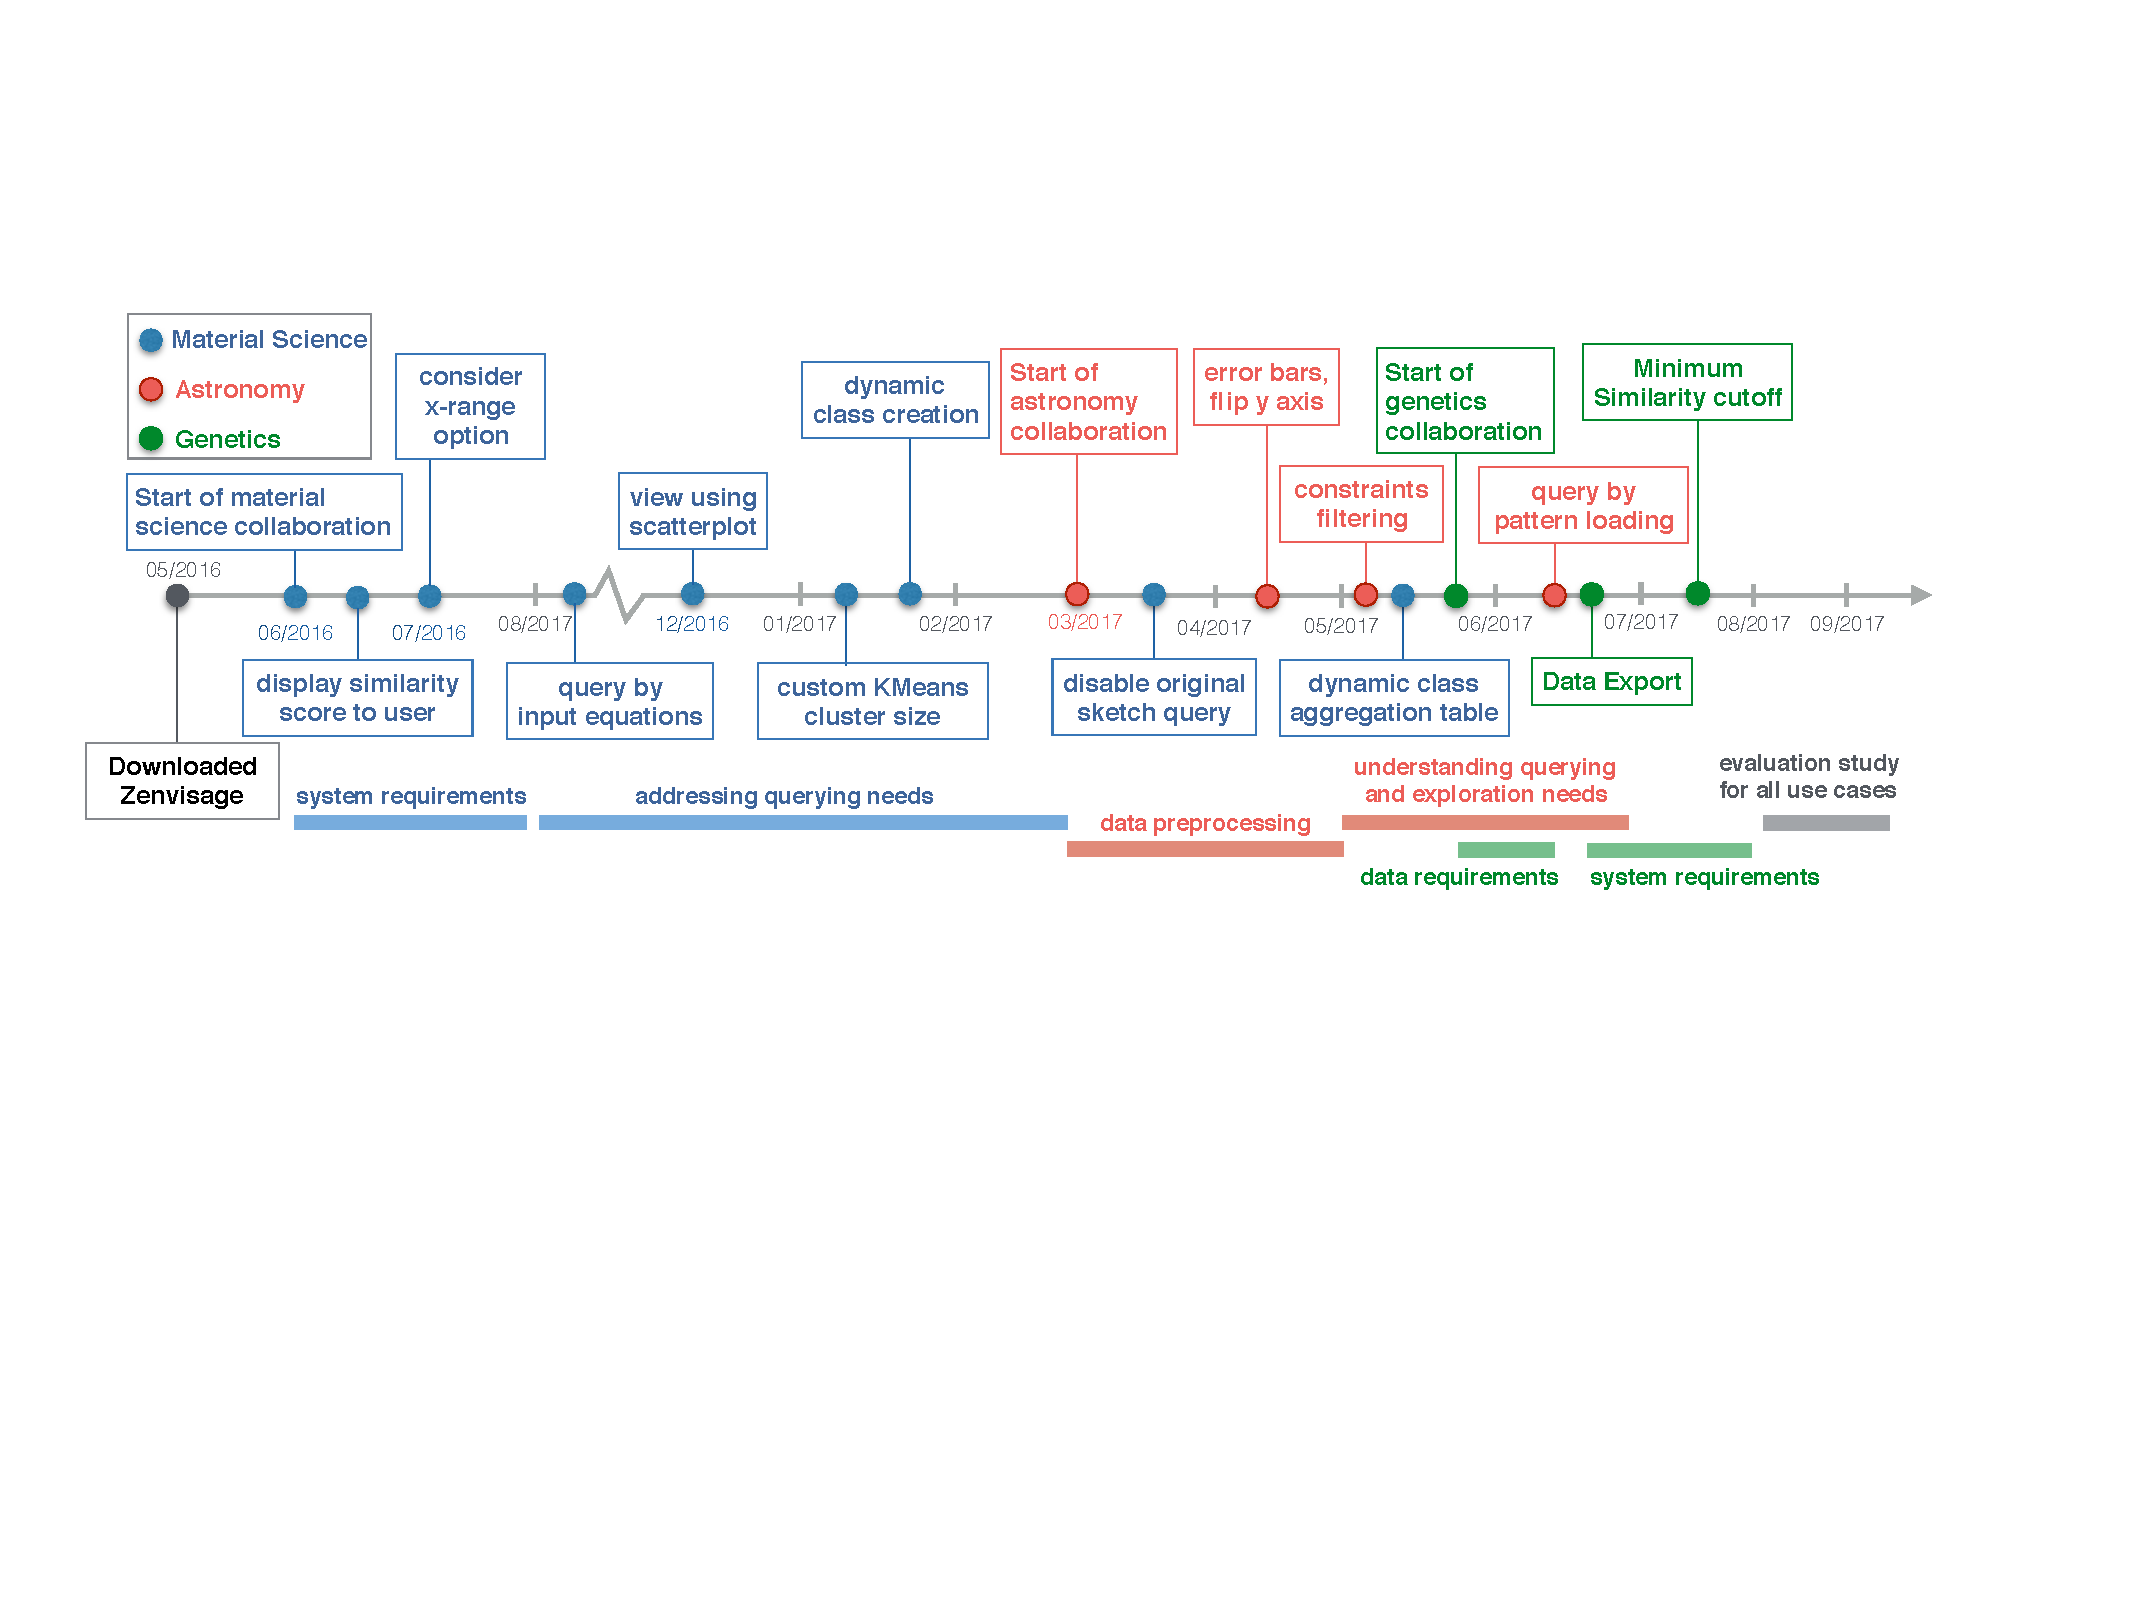
\includegraphics[width=6in]{figures/timeline.pdf}
	\vspace{-6pt}\caption{Timeline for progress in participatory design studies.}
	\label{timeline}
	\vspace{-10pt}
\end{figure*}

\begin{figure}[h!]
  \centering
  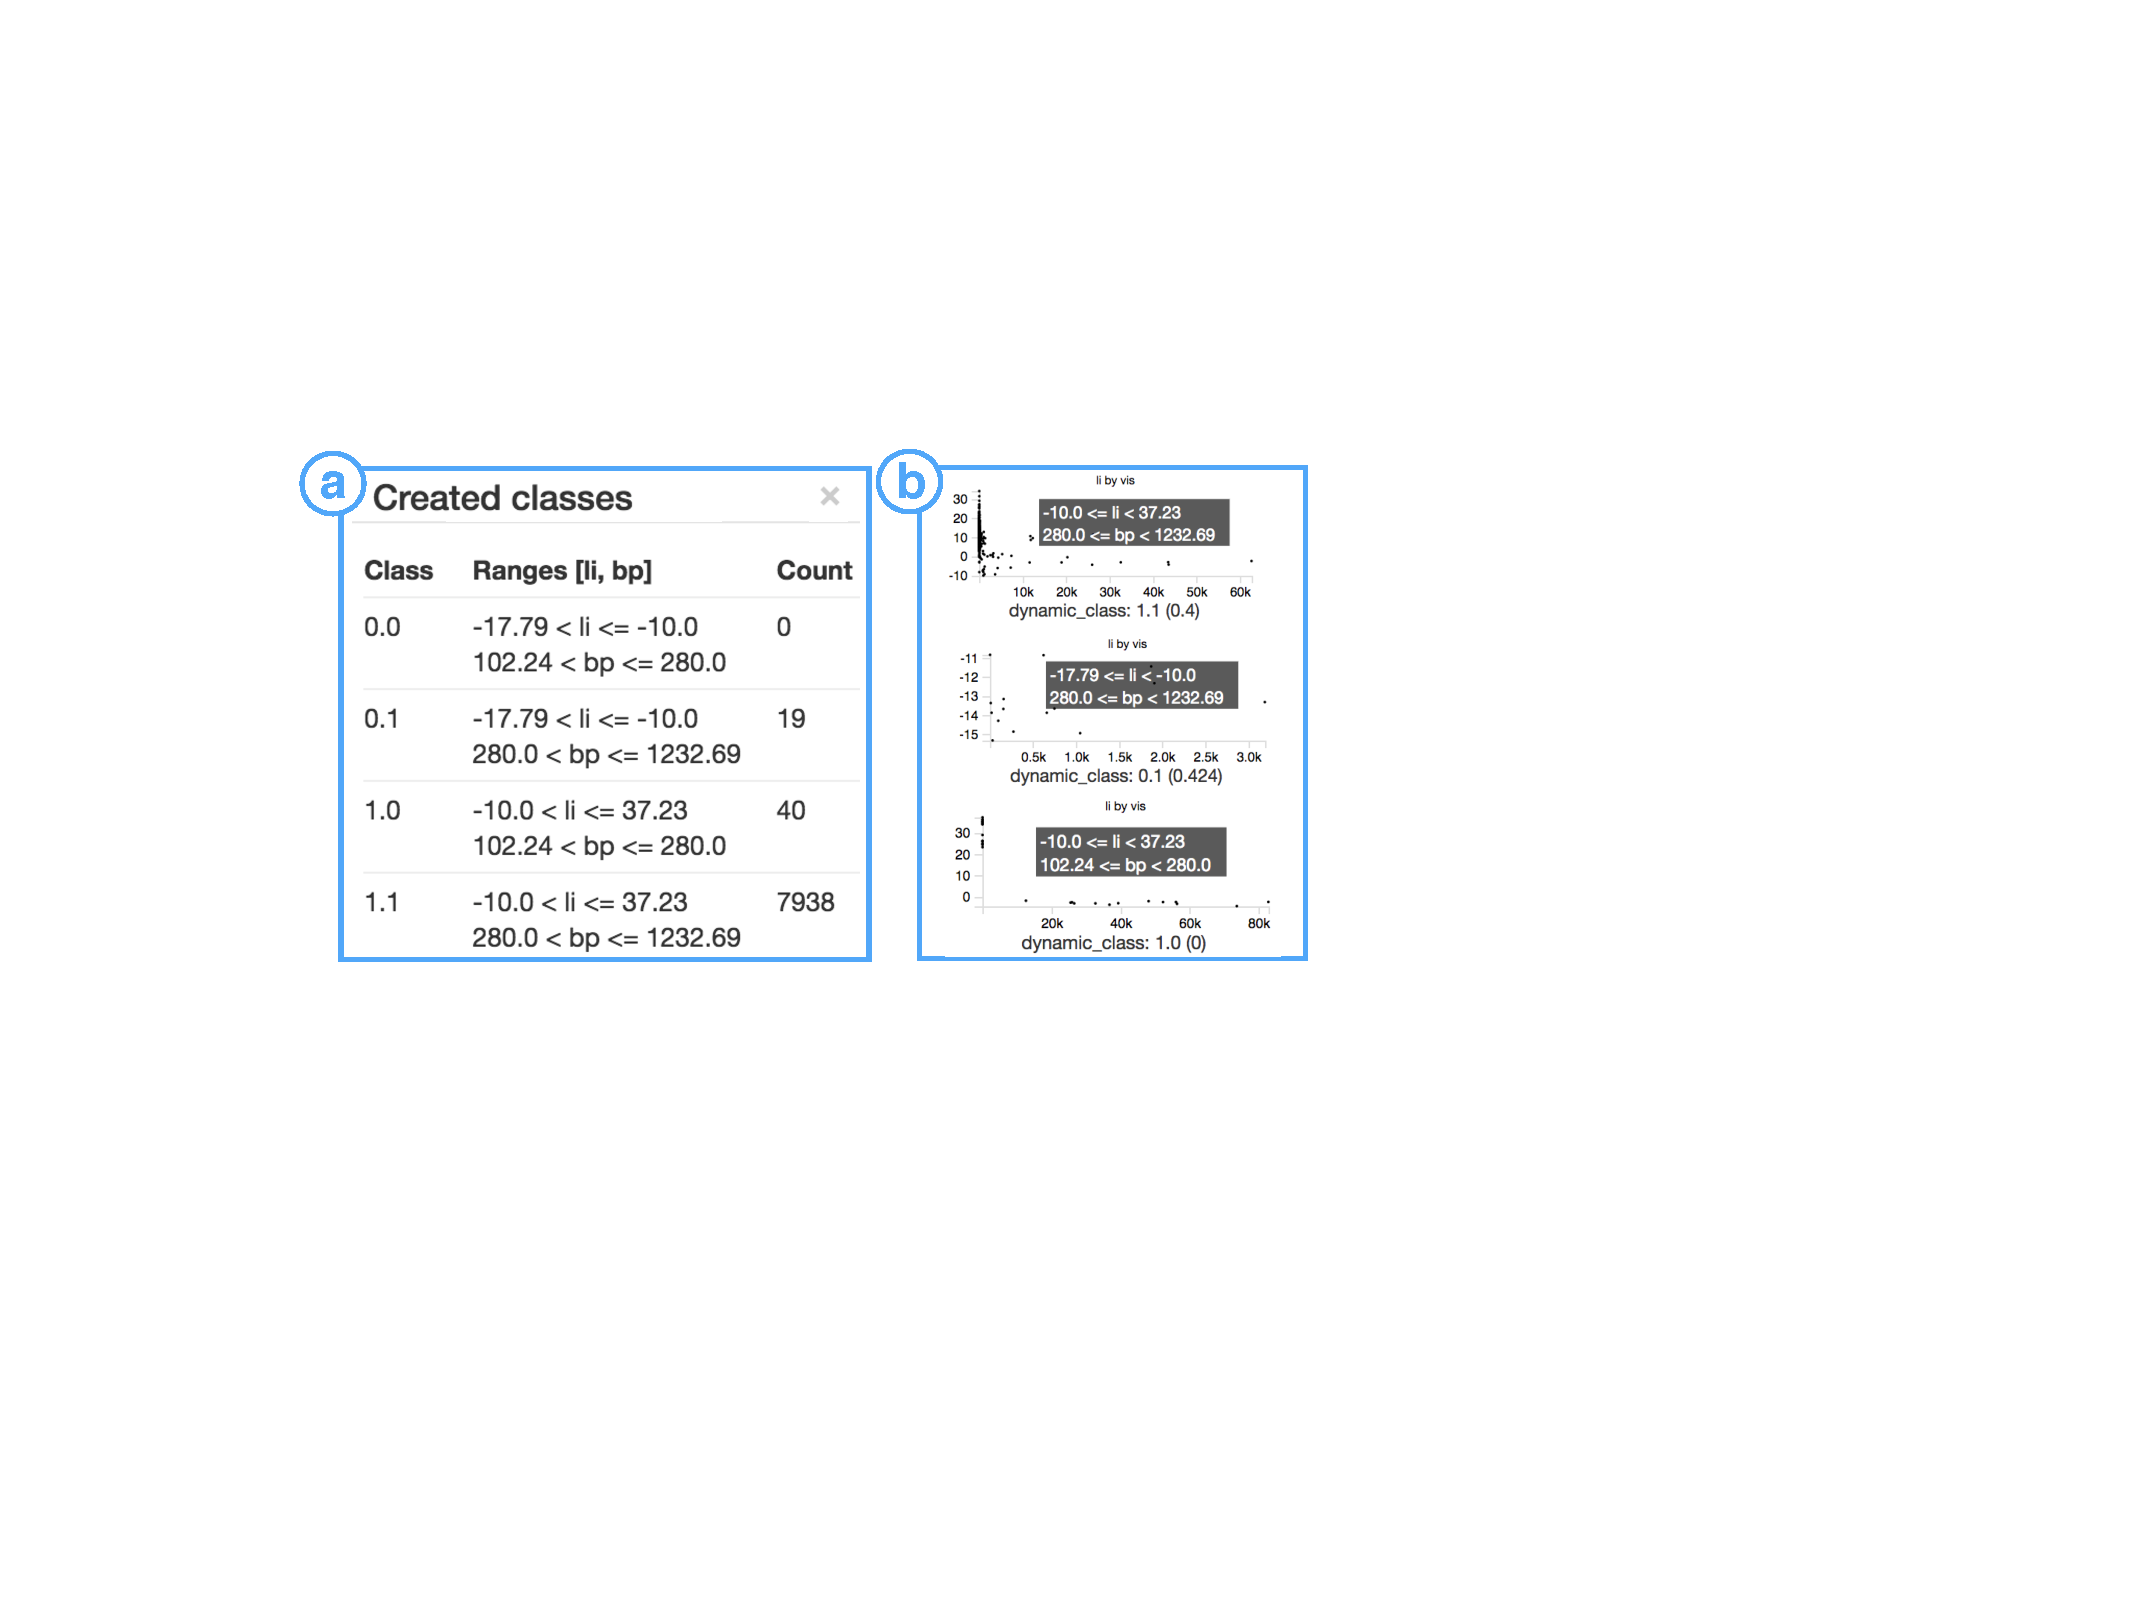
\includegraphics[width=0.95\linewidth]{figures/dcc.pdf}
  \vspace{-6pt}
  \caption{\change{Example of dynamic classes. (a) Four different classes with different Lithium solvation energies (li) and boiling point (bp) attributes based on user-defined data ranges. (b) Users can hover over the visualizations for each dynamic class to see the corresponding attribute ranges for each class. The visualizations of dynamic classes are aggregate across all the visualizations that lie in that class based on the user-selected aggregation method.}}
  \label{dcc}
  \vspace{-10pt}
\end{figure}
\begin{figure}[h!]
  \centering
  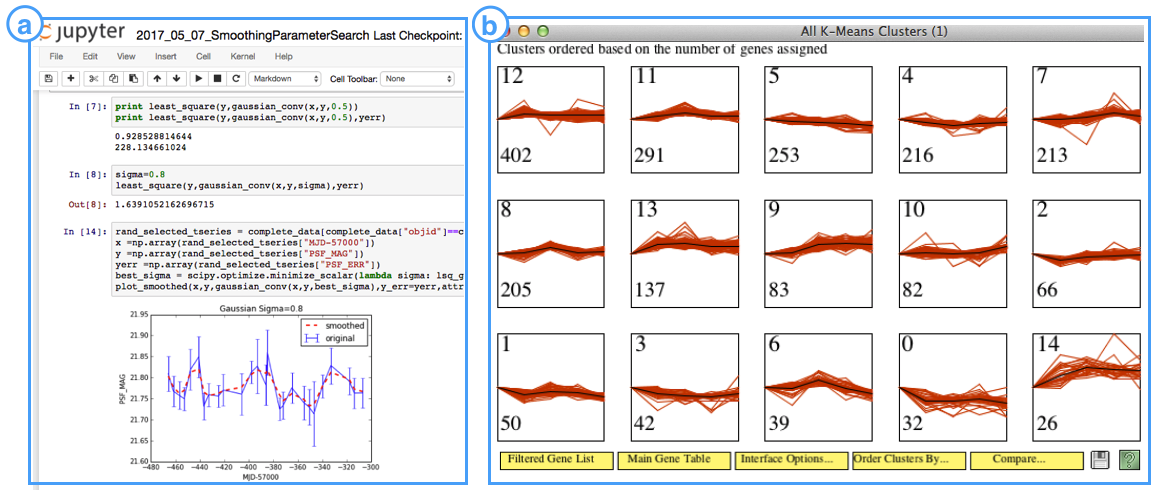
\includegraphics[width=\linewidth]{figures/workflow.png}
  \caption{Examples of the scientists' original workflow: a) A1 examines a light curve manually using the Jupyter notebook environment, b) G2 uses a domain-specific software to examine clustering outputs.}
  \label{workflow}
\end{figure}
\section{Evaluation Study Analysis Details\label{apdx:studydetails}}
We analyzed the transcriptions of the evaluation study recordings through open-coding and
categorized every event in the user study using the following coding labels:
\begin{denselist}
    \item Insight (Science) \textbf{[IS]}: Insight that connected back to the science (e.g. ``This cluster resembles a repressed gene.'')
    \item Insight (Data) \textbf{[ID]}: Data-related insights (e.g. ``A bug in my data cleaning code generated this peak artifact.'')
    \item Provoke (Science) \textbf{[PS]}: Interactions or observations that provoked a scientific hypothesis to be generated.
    \item Provoke (Data) \textbf{[PD]}: Interactions or observations that provoked further data actions to continue the investigation.
    \item Confusion \textbf{[C]}: Participants were confused during this part of the analysis.
    \item Want \textbf{[W]}: Additional features that participant wants, which is not currently available on the system.
    \item External Tool \textbf{[E]}: The use of external tools outside of \zvpp to complement the analysis process.
    \item Feature Usage \textbf{[F]}: One of the features in \zvpp was used.
    \item Session Break \textbf{[BR]}: Transition to a new line of inquiry.
\end{denselist}

\begin{table}[h!]
  \begin{tabular}{lrrrrrrrrr}
  \hline
   Domain           &   IS &   ID &   PS &   PD &   C &   W &   E &   BR &   F \\
  \hline
   astro            &    4 &   12 &   13 &   57 &   2 &  18 &  20 &   22 &  67 \\
   genetics         &    8 &   12 &    7 &   35 &   4 &  13 &   1 &   21 &  52 \\
   mat sci          &   14 &    8 &    7 &   44 &   8 &  11 &   3 &   12 &  48 \\
  \hline
  \end{tabular}
  \caption{Count summary of thematic event code across all participants of the same subject area.}
\end{table}

\npar In addition, based on the usage of each feature during the user study, we categorized the features into one of the three usage types:
\begin{denselist}
    \item Practical \textbf{[P]}: Features used in a sensible and meaningful way.
    \item Envisioned usage \textbf{[E]}: Features which could be used practically if the envisioned data was available or if they conducted downstream analysis, but was not performed due to the limited time during the user study.
    \item Not useful \textbf{[N]}: Features that are not useful or do not make sense for the participant's research question and dataset.
\end{denselist}
The feature usage labels for each user is summarized in Figure~\ref{feature_heatmap}. A feature is regarded as \emph{useful} if it has a \textbf{P} or \textbf{E} code label. Using the matrix from Figure~\ref{feature_heatmap}, we compute the percentage of useful features for each sensemaking process as: $\frac{\textrm{\# of useful features in process}}{\textrm{total \# of features in process} \times \textrm{total \# of users}}$.
\begin{figure}[h!]
    \centering
    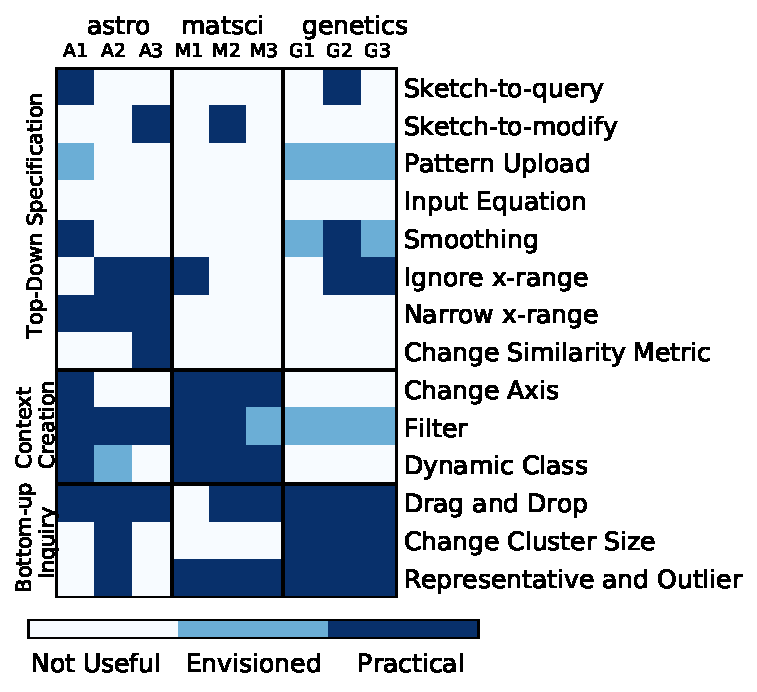
\includegraphics[width=0.75\columnwidth]{figures/PENcoding.pdf}
    \vspace{-6pt}\caption{Heatmap of features categorized as practical usage (P), envisioned usage (E), and not useful (N). Columns are arranged in the order of subject areas and the features are arranged in the order of the three foraging acts. We find that participants preferred to query using bottom-up methods such as drag-and-drop over top-down approaches such as sketching or input equations. Participants found that context creation via filter constraints and dynamic class creation were powerful ways to compare between subgroups or filtered subsets.}
    \label{feature_heatmap}
    \vspace{-5pt}
\end{figure}
